\documentclass[10pt, a4paper]{article}
\usepackage{lrec2016}
\usepackage{multibib}
\newcites{languageresource}{Language Resources}
\usepackage{graphicx} % for eps graphics
\usepackage{epstopdf}
\usepackage[latin1]{inputenc}

% Inari's additions
\usepackage[colorlinks=true,citecolor=blue,urlcolor=blue]{hyperref}
\usepackage{color}
\newcommand{\todo}[1]{{\color{cyan}\textbf{[TODO: }#1\textbf{]}}}
\usepackage{units} % for nicefrac
\usepackage{wasysym} % for clock

%%%%%%%%%%%%%%%%%%%%%%%%%%%%%%%%%%%%%%%%%%%%%%%%%%%%%%%%%%%%%%%%%%%%%%%%%%%
 
\title{Analysing Constraint Grammars with a SAT-solver}

\name{Inari Listenmaa, Koen Claessen}

\address{University of Gothenburg, Chalmers University of Technology \\
         Gothenburg, Sweden \\
         inari@chalmers.se, koen@chalmers.se\\}


\abstract{
We describe a method for analysing Constraint Grammars (CG) that can detect internal conflicts and redundancies in a given grammar, without the need for a corpus. The aim is for grammar writers to be able to automatically diagnose, and then manually improve their grammars. Our method works by automatically translating the given grammar into logical constraints that are analysed by a SAT-solver. We have evaluated our analysis on a number of non-trivial grammars and found inconsistencies.
\newline 
\Keywords{Constraint Grammar, SAT, Grammar Analysis} }

\begin{document}

\maketitleabstract

% Introduction & problem description
\section{Introduction}
\label{sec:intro}

Constraint Grammar (CG, \cite{karlsson1995constraint})
% \citep[CG][]{karlsson1995constraint} 
is a formalism for disambiguating morphologically analysed input.
CGs are valuable language resources for rule-based language processing, especially for lesser resourced languages. They are robust and require no extensive corpora or other language resources. The formalism is lightweight, and even small CGs are shown to be worthwile \cite{lene_trond2011}.

As CGs grow larger, .

\cite{bick2013tuning} presents efforts to optimise hand-written CGs using machine learning techniques.
While Bick's experiments show improvements in results, the grammar writer is none the wiser why is the grammar better.
Our toolset is designed to complement the existing efforts.
The ideal use case would be a grammar writer, who wants to know e.g.

\begin{itemize}
\item Is there a sentence that triggers rule(s) X but not rule(s) Y
\item Give a sentence that is ambiguous but doesn't trigger any rules
\item Does my grammar contain ``dead code'' -- rules that would not fire in any case?
\end{itemize}

The technique requires an existing morphological lexicon, but no corpus.
This makes it suitable also for languages without large corpora.
Authors writing grammars for well-resourced languages can also benefit from the technique, as an additional tool along with a gold standard corpus. 
Hand-annotated corpora are commonly used in the development of CGs, because they give immediate feedback whether a new rule increases or decreases accuracy, and by how large margin (\cite{voutilainen2004}). For a language with no free hand-tagged corpus available, \cite{tyers_reynolds2015} describe 

Things you can get from corpus:

\begin{itemize}
\item \# times the rule was applied
\item \% times it was correct
\end{itemize}
Strengths: gives concrete feedback about the effect of rules. Good especially at the beginning stages of grammar writing.

Things you can get from ML tuning:
\begin{itemize}
\item Variations in the place of the rule
\item Variations in the conditions (careful, ...) of the rule
\end{itemize}
Good side: try all combinations to find the best result.


Things you can get from SAT solver:
\begin{itemize}
\item Interaction of rules; 
\item Create word sequences to test what is possible and what can never happen
\end{itemize}


Given a large morphological lexicon, it is relatively easy to restrict each individual word to contain only realistic ambiguities. We expand the lexicon, map each wordform to its possible analyses, and then ignore the actual wordforms. For instance, a Spanish morphological lexicon contains the entries \texttt{casa:<verb><sg><p3>} and \texttt{casa:<noun><sg>}, hence we know that a confusion between a 3rd person singular verb and a singular noun is possible. The lexicon is not likely to contain a wordform that can be analysed both as an adjective and punctuation, so that kind of ambiguous word is never created.
However, since our method is corpus-free, it does not contain any restrictions as to what words can follow each other. \footnote{Encode morphological lexicon and CG rules in SAT + ask for a sentence that will trigger rules = natural language generation! \:D/}

\todo{Relate to conf themes: "Methodologies and tools for LRs construction and annotation" and
"Validation and quality assurance of LRs"}

% * Describe problem: CGs are huge & prone to mistakes,
%  * we are looking at conflicts such as ...
%  * if you forgot a case
%  * some evidence that big CGs have conflicts and this is a real problem
%  * Eckhard's paper to explain why conflicting rules are a problem
%  * Goal: help grammar writer while they are writing the grammar, to avoid these kinds of problems
%  * Examples

% * Describe the technique

% * Preliminary results
%  - dutch & spanish
%  - mention scalability
%  - talk about size of SAT problem -- give number of SAT clauses for the last rule in the biggest grammar I have

% * Future work
%  - analysing different grammar formalisms
%  - asking different questions
%  - restrict yourself to readings that are actually words





% Implementation details; very brief for the abstract
\section{Implementation}
\label{sec:implementation}

In this section, we describe the implementation of the toolset.
The SAT encoding we use is introduced in \cite{listenmaa_claessen2015}, along with a working CG compiler.
Since we want to test the rules in a way that doesn't depend on data, we operate on a \emph{symbolic sentence}: a word sequence which we can modify according to the properties we want to test.

\paragraph{SAT encoding of CG rules}

A single CG rule is a template which creates a concrete clause for each instance where it is applied.
%Each potential analysis is represented as a variable, and the rules are translated into clauses that operate on those variables.
Table~\ref{table:vars} shows the rule \texttt{REMOVE v IF (-1 det)} applied to the text \emph{the bear}.
The analyses of the word forms are represented as variables, and
the default rule ensures that each word has at least one analysis.
%This makes \texttt{the\_det} true by default, therefore the implication must hold, and \texttt{bear\_v\_pl} will be removed.
For more details about the encoding, see \cite{listenmaa_claessen2015}.

% table:vars moved to main file for positioning


\paragraph{Word-internal constraints}

The symbolic sentence consists of symbolic words.
In the beginning, a symbolic word is a list of all possible tag combinations, and we don't know which ones are true.
%These tag combinations may be underspecified for lemma or other features---similarly, a CG rule may target any noun, a plural noun or the noun \emph{bear}.
Given a large morphological lexicon, we can restrict the individual words to contain only realistic ambiguities. 
For instance, a Spanish morphological lexicon contains the entries \texttt{casa:casar<verb><sg><p3>} and \texttt{casa:casa<noun><sg>}, hence we know that a confusion between a 3rd person singular verb and a singular noun is possible. 
%The lexicon is not likely to contain a wordform that can be analysed both as an adjective and punctuation, so that kind of ambiguous word is never created.

%However, since our method is corpus-free, we don't add any external restrictions as to what words can follow each other.

\paragraph{Symbolic sentences}

We apply a concrete rule to a symbolic sentence
we get back a symbolic sentence: it's the same table except that 

we create a new variable for w2<verb> (target)a
 with the target changed into a new variable

definition of w2'<verb> = *nice formula*


Figure~\ref{fig:example} shows a fragment of of a two-word symbolic sentence, before and after applying the rule \texttt{REMOVE verb IF (-1 det)}\footnote{For simplicity, we don't show the word-internal constraints that come from the lexicon, but only the rule application.}.
As with real analyses, each tag combination is given a variable, and applying a rule means creating a concrete clause for each instance where a determiner is found preceding a verb.
In a symbolic sentence, every word has potentially every tag combination, and applying the rules will shape the sentence into something that respects the constraints of the language.

\begin{figure}[h]
\includegraphics[width=0.42\textwidth]{symbolic_sentence.png}
\caption{Symbolic sentence beginning to take shape \todo{make this less confusing?}}
\label{fig:example}
\end{figure}


The example rule states that the sentence may not have a verb after a determiner.
The variable \texttt{w2<verb>} is the situation of the second word's verb status before applying the rule. We create a new variable \texttt{w2'<verb>}, whose value depends on whether the condition holds (if \texttt{w1<det>} is true); whether it was true on the last round (if \texttt{w2<verb>} is already removed by another rule, \texttt{w2'<verb>} cannot reappear); and whether it is the only analysis left (not depicted in the picture).
All the analyses not targeted by this rule remain the same.


% \begin{figure}[]
% \includegraphics[width=0.42\textwidth]{symbolic_sentence.png}
% \caption{Symbolic sentence beginning to take shape \todo{make this less confusing?}}
% \label{fig:example}
% \end{figure}

%The applications of these rules shape our symbolic sentence into containing only things that can survive the rules. 

The effect of the old rule applications is retained when a new rule is added.
This means that we can ask a question ``after applying rules $0-i$, is it possible for $i+1$ to apply?'', and the answer is reliable; we cannot find a counterexample by just having a bit more data, because we start from literally all possibilities, and each rule restricts the set of possible sentences.
%If rule \texttt{r100} would require the first word to be a noun, and causes a conflict because it is not a noun, we know that it is because there is no way for w1 to be a noun.

%Note that this method is not suitable for language generation: rules in any realistic CG are tailored for real life ambiguities, whereas our symbolic sentence starts with literally all possibilities of tag combinations.

\paragraph{What kind of questions we can ask?}

The example so far has been of type ``Can rule Z apply after A-Y?''
In case a conflict is detected, we can dig into it and refine where the problem is: e.g. is the condition not met, or is it the case that the target is already removed or the only remaining analysis.
We can find what other rule or rules prevent others from applying, or if the conflict is rule-internal, such as nonexisting tag set or contradicting requirements of a context word (e.g. a word must be unambiguously two different POS).


In addition to analysing a whole grammar, 
we can construct all kinds of symbolic sentences to test out individual rules. 
We can set the length, restrict individual words (e.g. ``3rd word must be a noun''), require that it triggers some rule but not other. 
This functionality can aid the grammar writer in the process, to see if they have missed a case or defined the tagset correctly.








% Preliminary evaluation and future work
\section{Evaluation and Future Work}
\label{sec:eval}

We tested three grammars to find rules that cannot apply. The smallest grammar was Dutch, with 68 rules; second was Spanish with 279 rules, and the largest was Finnish, with 1185 rules.
For the smaller grammars, we were able to verify manually that the results are true.

\begin{table}[]
\centering
\begin{tabular}{|l|l|l|l|}
\hline
                      & \textsc{nld}  & \textsc{spa}  & \textsc{fin}  \\ \hline
Rules in grammar      & 68              & 279               & 1185              \\ \hline
Redundant rules found & 1               & ???               & ???    \\ \hline
Running time          & 7s              & 3min 22s          & 3h 26min    \\ \hline
\end{tabular}
\caption{Results}
\label{table:res}
\end{table}

\todo{Other things we found from the grammar:}
With the Spanish grammar, the method pointed us to a nonsensical set definition.
\texttt{w2<n><np><adj><det><preadv><adv><vblex><vbmod><vbhaver><vbser><prn><pr><cnjcoo><cnjsub><cnjadv><rel><ij>}

For future work, we want to improve the performance and scale up to larger grammars, and handle the full expressivity of CG-3, with \textsc{map}, \textsc{add} and \textsc{substitute} rules.
We want to also ask different questions, such as \todo{...}.
Finally, we want to test the approach to other grammar formalisms.



% * Preliminary results
%  - dutch & spanish
%  - mention scalability
%  - talk about size of SAT problem -- give number of SAT clauses for the last rule in the biggest grammar I have

% * Future work
%  - analysing different grammar formalisms
%  - asking different questions
%  - restrict yourself to readings that are actually words

\section*{Acknowledgments}
We thank Eckhard Bick for the idea to apply SAT to CG analysis, and Francis Tyers for insightful discussions.

\section{Bibliographical References}
\label{main:ref}

\bibliographystyle{lrec2016}
\bibliography{../cg}


% \section{Language Resource References}
% \label{lr:ref}
% \bibliographystylelanguageresource{lrec2016}
% \bibliographylanguageresource{cg}

\end{document}
